\chapter{Einleitung}
\pagenumbering{arabic}
\section{Aufgabenstellung gemäss Eingabe}
Im Dokument 'Bachelorthesis-Aufgabe ist' folgendes festgehalten:
\begin{quote}
Seit mehreren Jahren bestreitet die HFTM unter der Leitung von Alain Rohr mit dem Solidus Team erfolgreich die internationalen Meisterschaften des RoboCups in der 'Logistics League'.
Das Team kennt sich meisterlich mit der Ansteuerung der Hardware aus, bittet aber die BFH um Mithilfe beim Software-Engineering.
Die Aufgabe dieser Arbeit ist es, ein Software-Design für die einzelnen Komponenten des verwendeten Roboters zu entwerfen. Angelehnt an die Vorgehensweise 'Domain Driven Design' soll konkret anhand des LIDARS gezeigt werden, wie das erarbeitete Software-Design implementiert und genutzt werden soll. Folgende Merkmale soll das Design mindestens aufweisen:

\begin{itemize}
	\item Die Schnittstelle der einzelnen Domänen muss Programmiersprachen-agnostisch sein
	\item Die Domänen müssen abgekapselt und unabhängig entwickelt und getestet werden können
	\item Das Design muss klar vorsehen, dass jedes Jahr das Entwicklungsteam komplett ausgetauscht wird
\end{itemize}
Bei dieser Arbeit gilt es auch zu beachten, dass die Software-Fähigkeiten des jeweiligen Entwicklungsteams erst noch ausgebildet werden müssen, es also nötig ist, die Schnittstellen so leicht und verständlich wie möglich zu halten, um nicht eine zu steile Lernkurve als Voraussetzung zu erschaffen.
\end{quote}
Im Kapitel \ref{sec:aufgabenstellung-messbar} wird die Messbare Aufgabenstellung (TODO) erläutert.

\section{HFTM Robocup}
\begin{figure}[htbp]
	\centering
	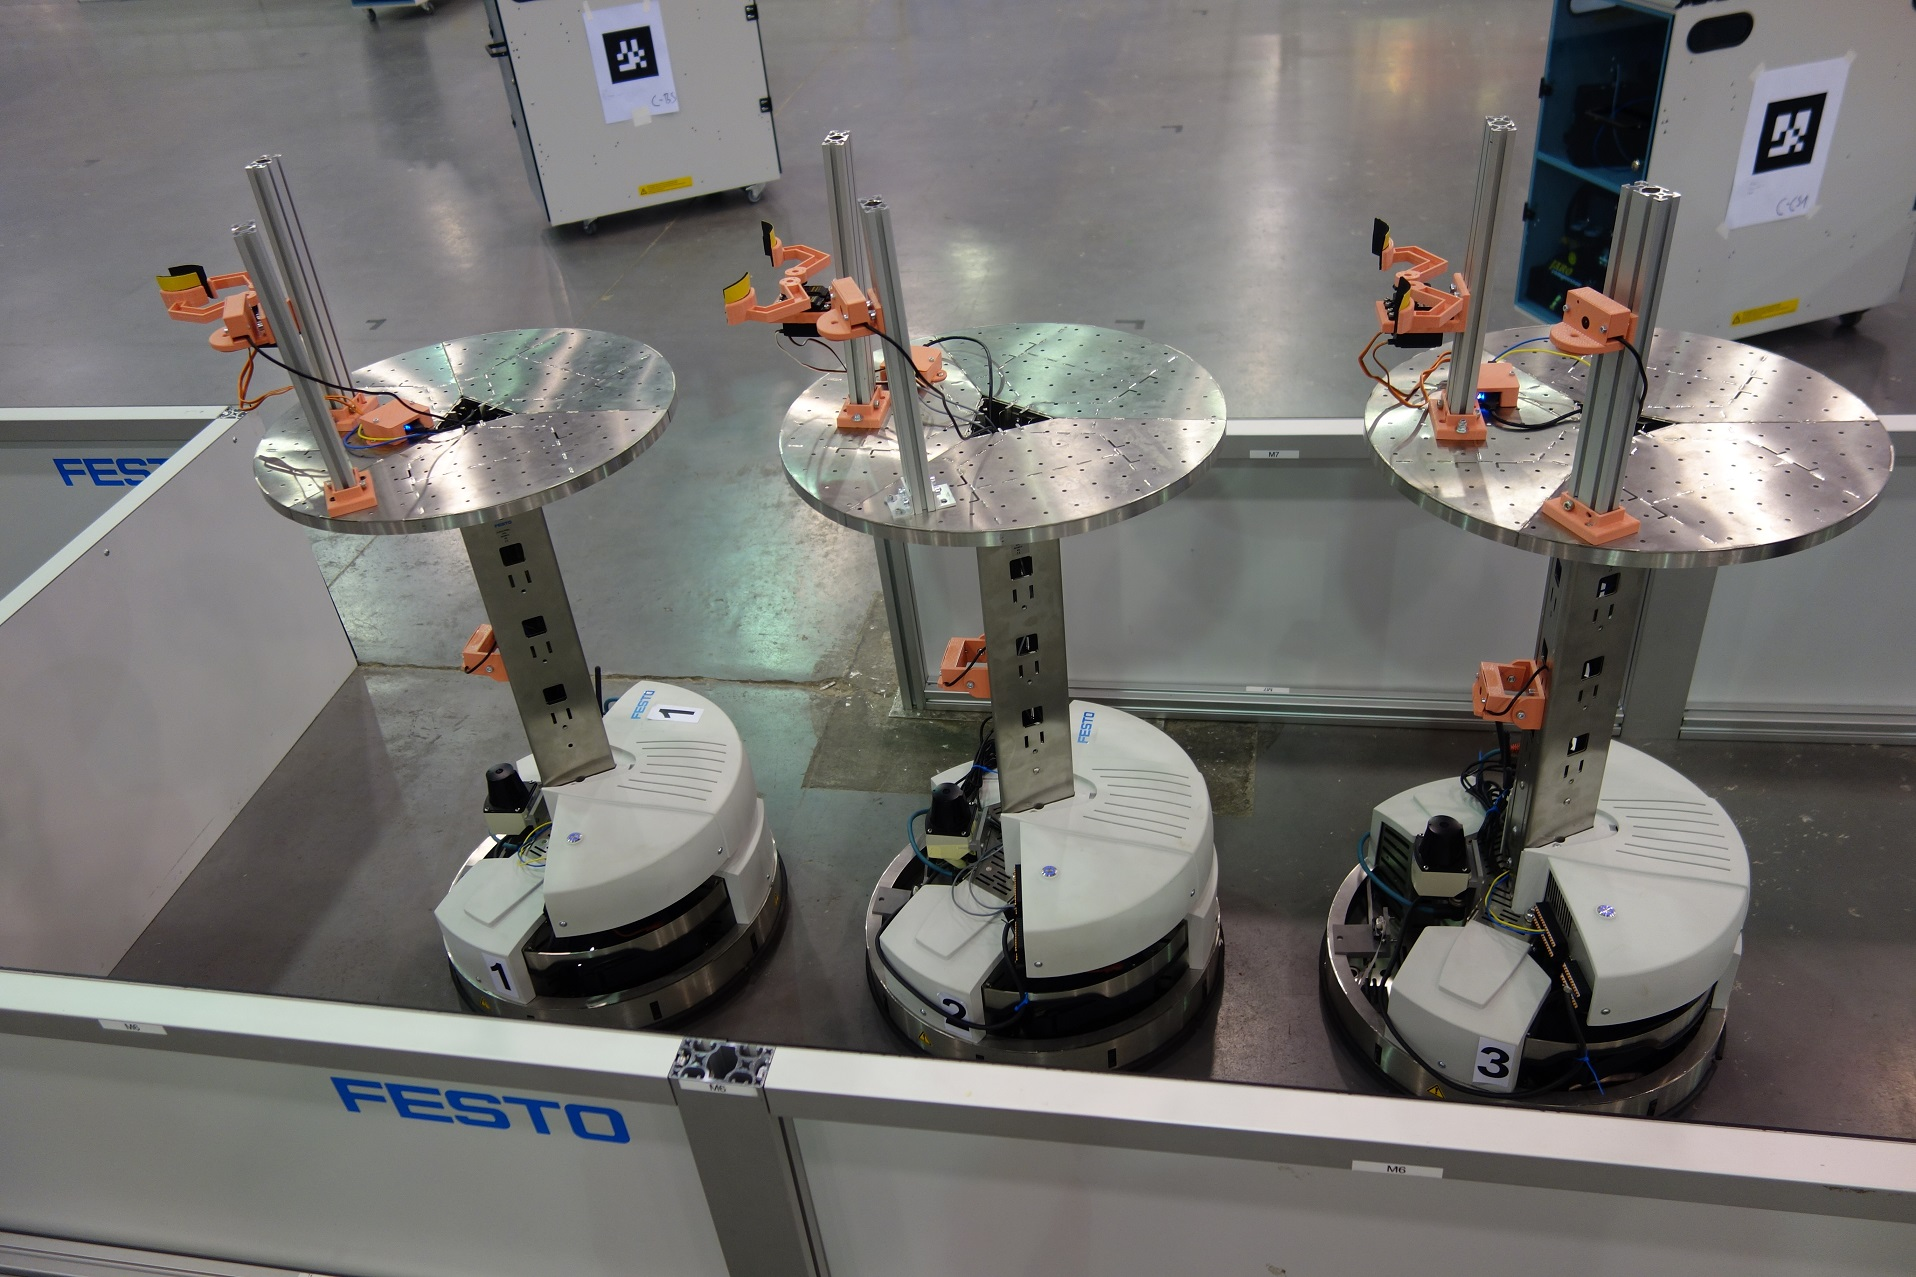
\includegraphics[width=0.5\textwidth]{img/robocup/robotino_v3.jpg}
	\caption{ein Bild\cite{robotino}}  
\end{figure}

TODO:
Roboter erklären, Schule erklären, Studienrichtung?

\section{Lidar}
TODO:
was ist \acrshort{lidar}, wozu wird es verwendet, Funktionsweise High-Level




